\documentclass{beamer}
\usepackage{listings}
\usepackage{color}
\usepackage{amsmath}
\usepackage{gvv}

\title{Area of Parallelogram}
\author{EE25BTECH11008 - Anirudh M Abhilash}
\date{September 16, 2025}

\begin{document}

%----------------- Title -------------------
\begin{frame}
\titlepage
\end{frame}

%----------------- Problem -------------------
\begin{frame}{Problem Statement}
The two adjacent sides of a parallelogram are 
\begin{align*}
\vec{a} = \myvec{2 \\ -4 \\ -5},  
\vec{b} = \myvec{2 \\ 2 \\ 3}
\end{align*}
Find the two unit vectors parallel to its diagonals. Using the diagonal vectors, find the area of the parallelogram.
\end{frame}

%----------------- Solution -------------------
\begin{frame}{Solution}
Diagonals:
\begin{align}
\vec{d}_1 = \vec{a} + \vec{b} \\
\vec{d}_2 = \vec{a} - \vec{b} \\
\vec{d}_1 = \myvec{4 \\ -2 \\ -2} \\ 
\vec{d}_2 = \myvec{0 \\ -6 \\ -8} 
\end{align}

Norms:
\begin{align}
\|\vec{d}_1\|^2 = \vec{d}_1^\top \vec{d}_1 = 24 \\
\|\vec{d}_1\| = 2\sqrt{6} \\
\|\vec{d}_2\|^2 = \vec{d}_2^\top \vec{d}_2 = 100 \\
\|\vec{d}_2\| = 10
\end{align}
\end{frame}

%----------------- Solution (cont) -------------------
\begin{frame}{Solution (cont..)}
Unit vectors along diagonals:
\begin{align}
\vec{u}_1 = \frac{\vec{d}_1}{\|\vec{d}_1\|}
= \frac{1}{2\sqrt{6}}\myvec{4 \\ -2 \\ -2} \\
\vec{u}_2 = \frac{\vec{d}_2}{\|\vec{d}_2\|} 
= \frac{1}{10}\myvec{0 \\ -6 \\ -8}.
\end{align}

Area of the parallelogram:
\begin{align}
\|\vec{a}\times\vec{b}\|^2 
= (\vec{a}^\top\vec{a})(\vec{b}^\top\vec{b}) - (\vec{a}^\top\vec{b})^2.
\\\vec{a}^\top\vec{a} = 45, 
\quad 
\vec{b}^\top\vec{b} = 17, 
\quad 
\vec{a}^\top\vec{b} = -19.
\\
\|\vec{a}\times\vec{b}\|^2 = 45 \cdot 17 - (-19)^2 = 404,
\\
\text{Area} = \sqrt{404} = 2\sqrt{101}.
\end{align}
\end{frame}

\begin{frame}{Solution (cont..)}


\begin{align*}
\boxed{\vec{u}_1 = \tfrac{1}{2\sqrt{6}}\myvec{4 \\ -2 \\ -2}, 
\quad 
\vec{u}_2 = \tfrac{1}{10}\myvec{0 \\ -6 \\ -8}, 
\quad 
\text{Area} = 2\sqrt{101}}
\end{align*}
\end{frame}

\begin{frame}[fragile]{Python Code (Plotting Parallelogram)}
\begin{lstlisting}[language=Python]
import numpy as np
import matplotlib.pyplot as plt
from mpl_toolkits.mplot3d.art3d import Poly3DCollection

A = np.array([2, -4, -5])
B = np.array([2,  2,  3])
O = np.array([0, 0, 0])
C = A + B
points = np.array([O, A, C, B])

fig = plt.figure()
ax = fig.add_subplot(111, projection='3d')
verts = [[O, A, C, B]]

\end{lstlisting}
\end{frame}

\begin{frame}[fragile]{Python Code (cont..)}
\begin{lstlisting}[language=Python]
ax.add_collection3d(Poly3DCollection(verts, alpha=0.3, facecolor='cyan'))
edges = [(O, A), (O, B), (A, C), (B, C)]
for p1, p2 in edges:
    ax.plot(*zip(p1, p2), color='blue')
ax.plot(*zip(O, C), color='red', linestyle='--')
ax.plot(*zip(A, B), color='green', linestyle='--')
labels = {"O": O, "A": A, "B": B, "C": C}
for name, coord in labels.items():
    ax.scatter(*coord, color='black', s=10)
    ax.text(coord[0], coord[1], coord[2], f"{name}{tuple(coord)}", fontsize=9)

\end{lstlisting}
\end{frame}

\begin{frame}[fragile]{Python Code (cont..)}
\begin{lstlisting}[language=Python]
ax.set_xlabel('X')
ax.set_ylabel('Y')
ax.set_zlabel('Z')

max_range = np.array([points[:,0].max()-points[:,0].min(), 
                      points[:,1].max()-points[:,1].min(), 
                      points[:,2].max()-points[:,2].min()]).max() / 2.0
mid_x = (points[:,0].max()+points[:,0].min()) * 0.5
mid_y = (points[:,1].max()+points[:,1].min()) * 0.5
mid_z = (points[:,2].max()+points[:,2].min()) * 0.5
ax.set_xlim(mid_x - max_range, mid_x + max_range)
ax.set_ylim(mid_y - max_range, mid_y + max_range)
ax.set_zlim(mid_z - max_range, mid_z + max_range)

plt.show()

\end{lstlisting}
\end{frame}

%----------------- Plot -------------------
\begin{frame}[fragile]{Plot}
\begin{figure}[H]\centering
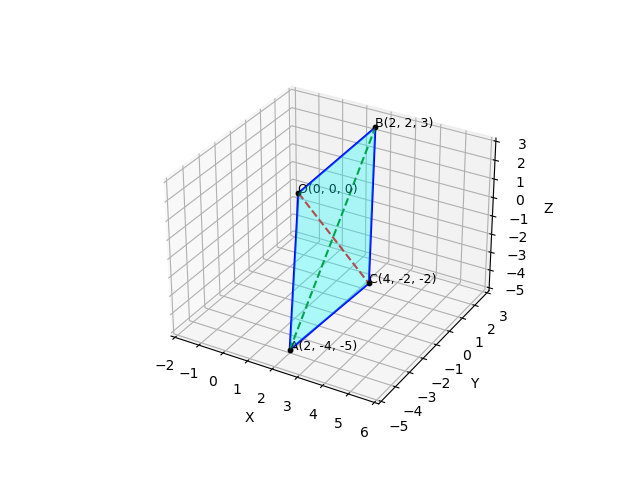
\includegraphics[width=1\columnwidth]{figs/plt.png}
\caption{Parallelogram along with diagonal vectors}
\label{fig:plt}
\end{figure}
\end{frame}

%----------------- C Code -------------------

\begin{frame}[fragile]{C Code (Computations)}
\begin{lstlisting}[language=C]
#include <math.h>
void diagonals(double A[3], double B[3], double d1[3], double d2[3]) {
    d1[0] = A[0] - B[0];
    d1[1] = A[1] - B[1];
    d1[2] = A[2] - B[2];

    d2[0] = A[0] + B[0];
    d2[1] = A[1] + B[1];
    d2[2] = A[2] + B[2];
}
double dot(double a[3], double b[3]) {
    return a[0]*b[0] + a[1]*b[1] + a[2]*b[2];
}
\end{lstlisting}
\end{frame}

\begin{frame}[fragile]{C Code (Cont..)}
\begin{lstlisting}[language=C]
void unit(double v[3], double u[3]) {
    double mag = sqrt(dot(v, v));
    u[0] = v[0]/mag;
    u[1] = v[1]/mag;
    u[2] = v[2]/mag;
}
double cross_via_dot(double a[3], double b[3]) {
    double mag_a2 = dot(a, a);
    double mag_b2 = dot(b, b);
    double dot_ab = dot(a, b);
    return sqrt(mag_a2 * mag_b2 - dot_ab * dot_ab);
}
\end{lstlisting}
\end{frame}


%----------------- Python Code -------------------
\begin{frame}[fragile]{Python Code (Calling C)}
\begin{lstlisting}[language=Python]
import ctypes

lib = ctypes.CDLL("./computations.so")
DoubleArray3 = ctypes.c_double * 3

lib.diagonals.argtypes = [DoubleArray3, DoubleArray3, DoubleArray3, DoubleArray3]
lib.unit.argtypes = [DoubleArray3, DoubleArray3]
lib.dot.argtypes = [DoubleArray3, DoubleArray3]
lib.dot.restype = ctypes.c_double
lib.cross_via_dot.argtypes = [DoubleArray3, DoubleArray3]
lib.cross_via_dot.restype = ctypes.c_double
\end{lstlisting}
\end{frame}


\begin{frame}[fragile]{Python Code (cont..)}
\begin{lstlisting}[language=Python]
A = DoubleArray3(2, -4, -5)
B = DoubleArray3(2, 2, 3)

d1, d2 = DoubleArray3(), DoubleArray3()
lib.diagonals(A, B, d1, d2)

u1, u2 = DoubleArray3(), DoubleArray3()
lib.unit(d1, u1)
lib.unit(d2, u2)

area = 0.5 * lib.cross_via_dot(d1, d2)

print("u1:", list(u1))
print("u2:", list(u2))
print("Area:", area)
\end{lstlisting}
\end{frame}

\end{document}